\begin{frame}
\frametitle{Checking for Emptiness}

\begin{figure}
\begin{center}
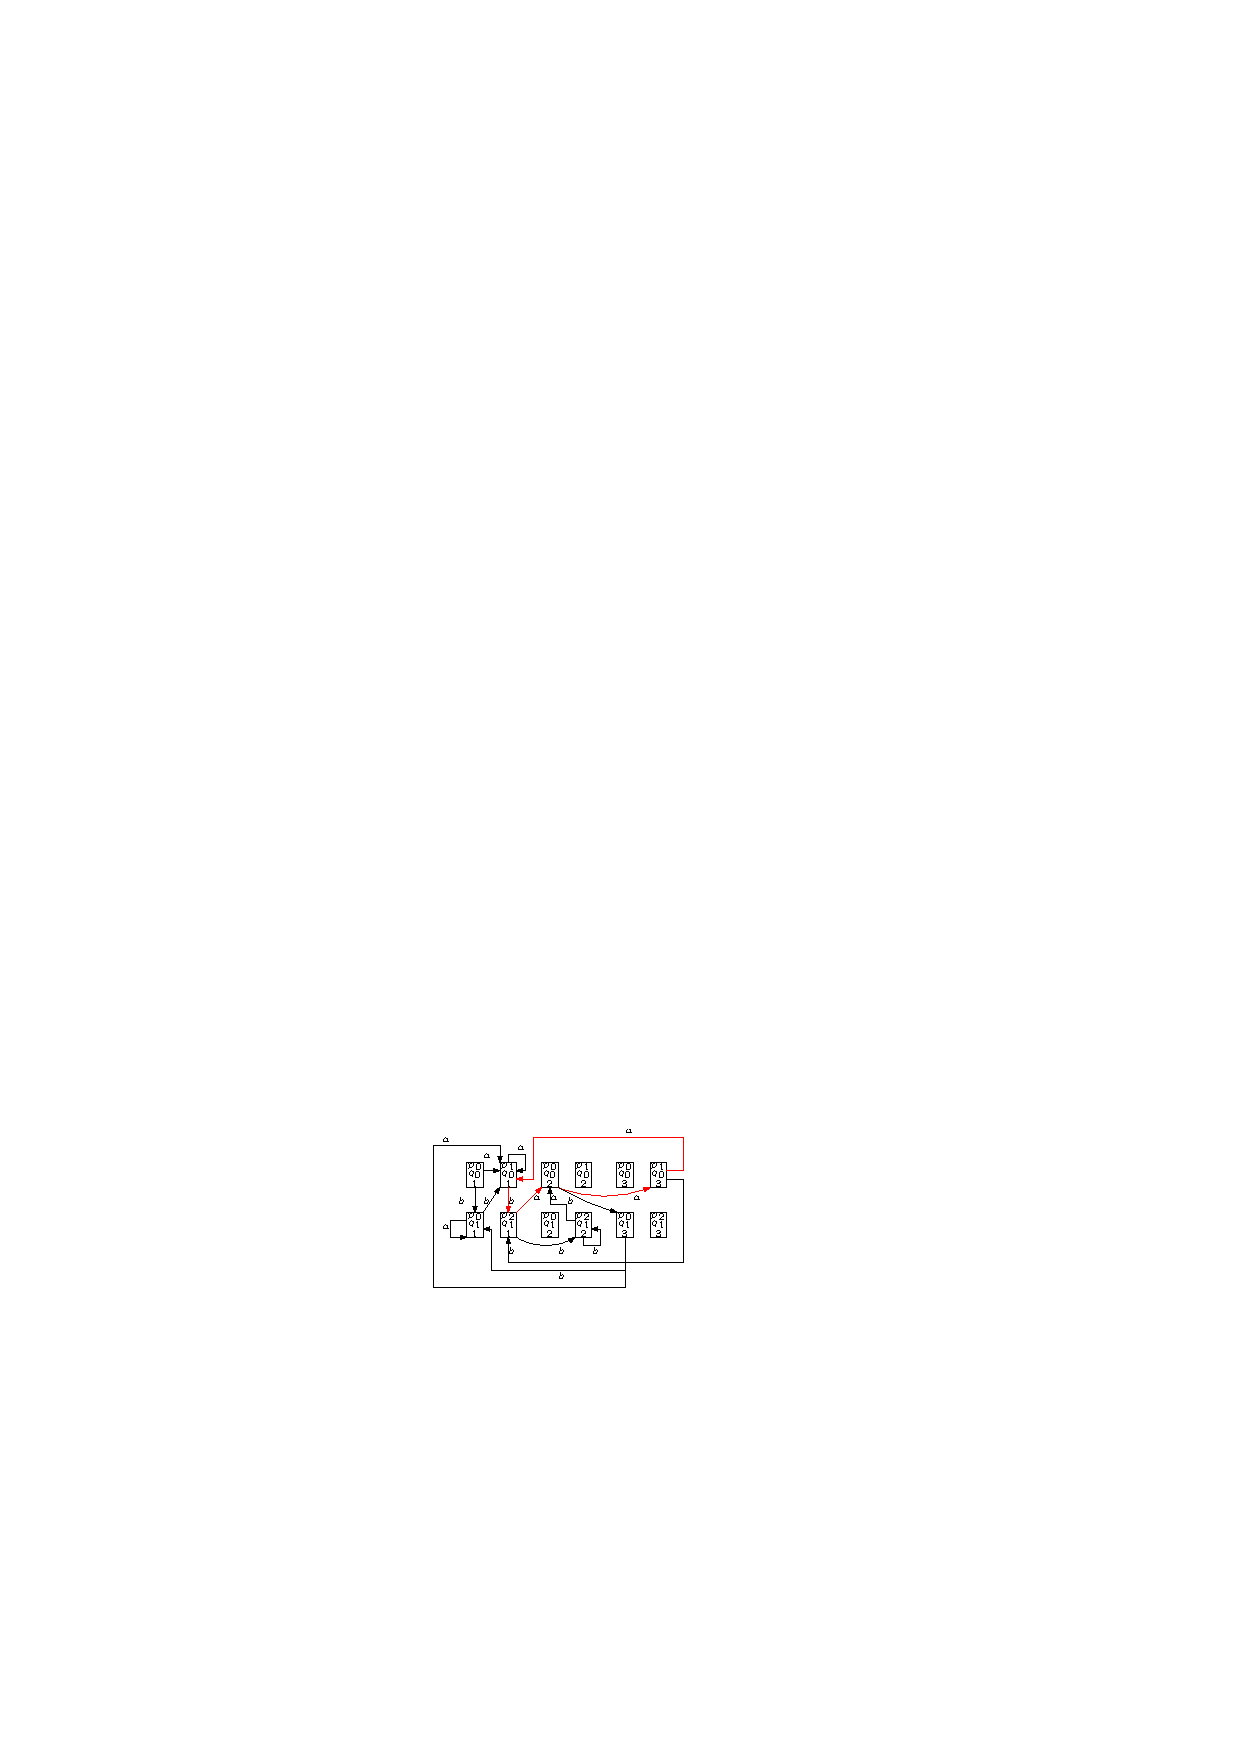
\includegraphics[width=45mm]{state_copy_transition_cycle.pdf}
\end{center}
%\vspace{-0.1in}
\caption{{\em \tiny{\textcolor{blue}{Cycle on the Intersection automata}}}}
\label{transition}
\end{figure}

\tiny{\textcolor{blue}{ The diagram depicts that:}}

\begin{itemize}
 \item \tiny{\textcolor{blue}{ There are multiple cycles in the intersection automata}}
 \item \tiny{\textcolor{blue}{ Cycle containing one representative accepting state from each control loop (e.g.
                      $\langle p_0, q_0, 1 \rangle \rightarrow \langle p_1, q_0, 1 \rangle \rightarrow \langle p_0, q_1, 1\rangle \dots)$. will be a valid run}} 
\item  \tiny{\textcolor{blue}{Necessary to examine each cycle to check for existence of at least one accepting state from each control
       loop}}
\end{itemize}  




\end{frame}